
\section{Methods}

\par We begin with a graphical exploration of our data. Box plots of $Age$, $BooksInPastYear$, and $log(BooksInPastYear)$ against $AnthClimateChangeReal$ are shown in Figure \ref{fig:EDA_boxplots}. The log transformation on $BookInPastYear$ appears to improve its distribution, so we use this transformed variable for our analysis.\footnote{The uppermost values of $BooksInPastYear$ are quite suspect, but we have no other reason to believe they are false, so we will leave them be.} Both pairs of means look somewhat different, so we will pay close attention to $Age$ and $log(BooksInPastYear)$ going forward.

\begin{figure}[h]
    \centering
    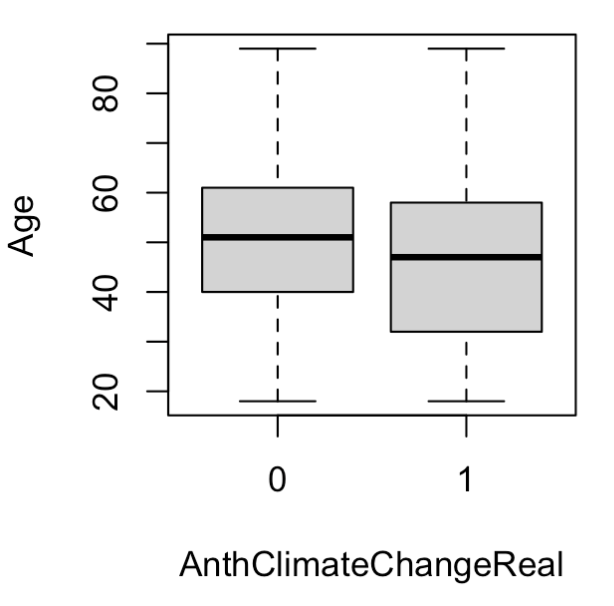
\includegraphics[scale=.45]{boxplot_age_anth.png}
    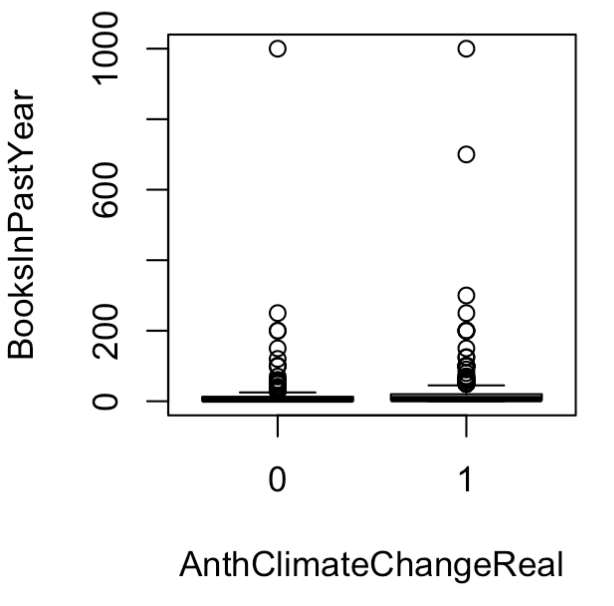
\includegraphics[scale=.45]{boxplot_books_anth.png}
    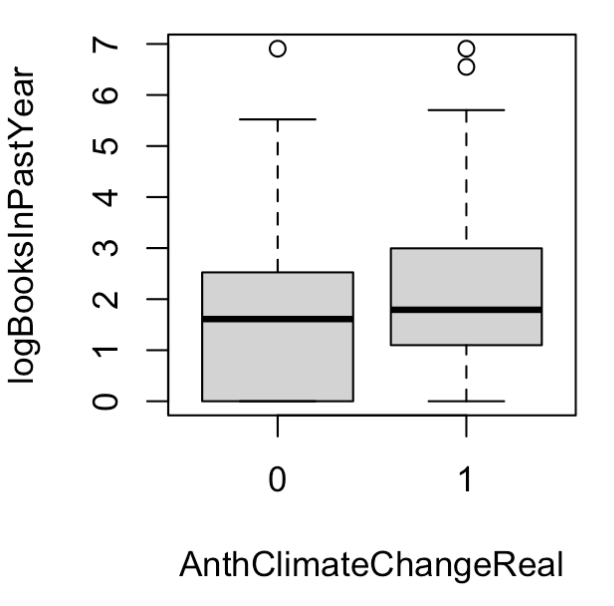
\includegraphics[scale=.45]{boxplot_logbooks_anth.png}
    \caption{Box plots of $Age$, $BooksInPastYear$, and $log(BooksInPastYear)$ vs. $AnthClimateChangeReal$}
    \label{fig:EDA_boxplots}
\end{figure}

\par We analyze potential effects of our binary variables by looking at tables of each against $AnthClimateChangeReal$. The percent of each level that reported belief in anthropogenic climate change for each variable is shown in Table \ref{tab:EDA_tables}. We see a significant gap in these percentages for $ScientistsGood$ and $SmartSadDumbHappy$, and moderately large gaps for $Male$, $VaccinesGood$, $College$, and $Married$. Even $HasSeenTransformers$ and $BelievesInGhosts$ look like they have potential to be significant. We will keep these rough rankings in mind as we proceed.

\par \bigskip Since we have only two quantitative variables left in consideration, we can plot each against all binary variables to check for potential interactions. As Figure \ref{fig:EDA_intx} shows, only four of these plots seem to have significantly different slopes for the two levels: $Age$ against $Male$, $HasSeenTransformers$, and $BelievesInGhosts$; and $log(BooksInPastYear)$ against $Married$. We will include these four interactions in the variables we test as we build our model.

\newpage

\begin{table}[h]
    \centering
    \begin{tabular}{|l|c|c|}
        \hline
        \textbf{Variable} & \textbf{0} & \textbf{1}\\
        \hline
        $ScientistsGood$ & 0.421 & 0.715\\
        $SmartSadDumbHappy$ & 0.572 & 0.717\\
        \hline
        $Male$ & 0.689 & 0.589\\
        $VaccinesGood$ & 0.577 & 0.653\\
        $College$ & 0.582 & 0.657\\
        $Married$ & 0.684 & 0.601\\
        \hline
        $HasSeenTransformers$ & 0.610 & 0.667\\
        $BelievesInGhosts$ & 0.620 & 0.676\\
        \hline
        $JobWillBeAutomated$ & 0.633 & 0.677\\
        $ShowerPeeingOk$ & 0.655 & 0.625\\
        \hline
    \end{tabular}
    \caption{Ratio of anthropogenic climate change belief for each level of our binary variables}
    \label{tab:EDA_tables}
\end{table}

\vspace{.4in}

\begin{figure}[!h]
    \centering
    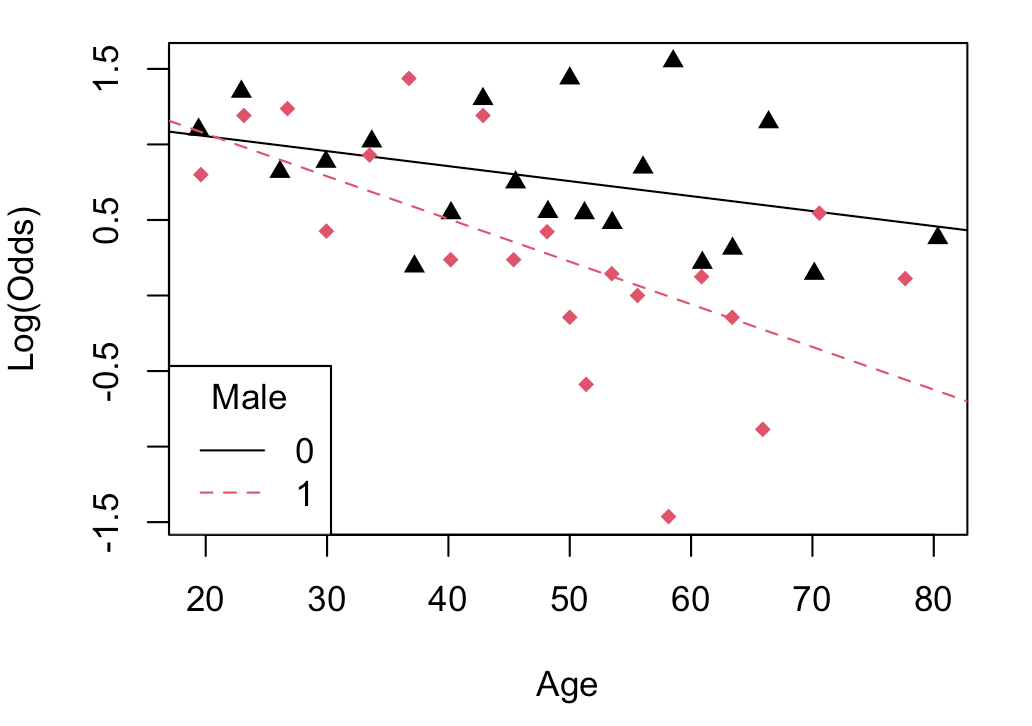
\includegraphics[scale=.3]{intxplot_age_male.png}
    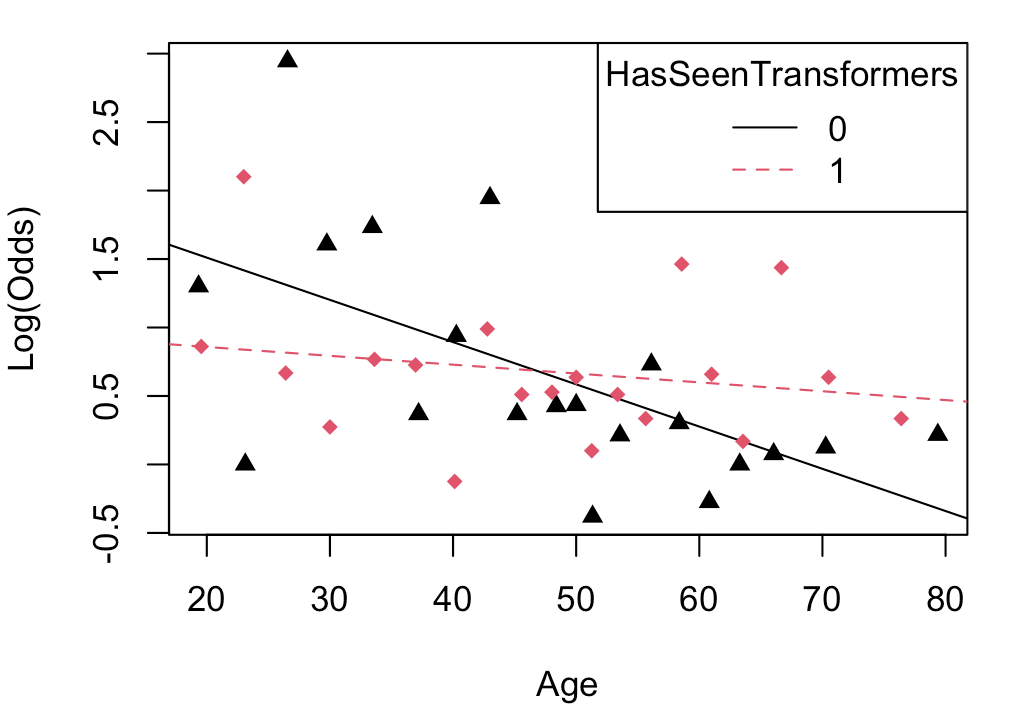
\includegraphics[scale=.3]{intxplot_age_transformers.png}
    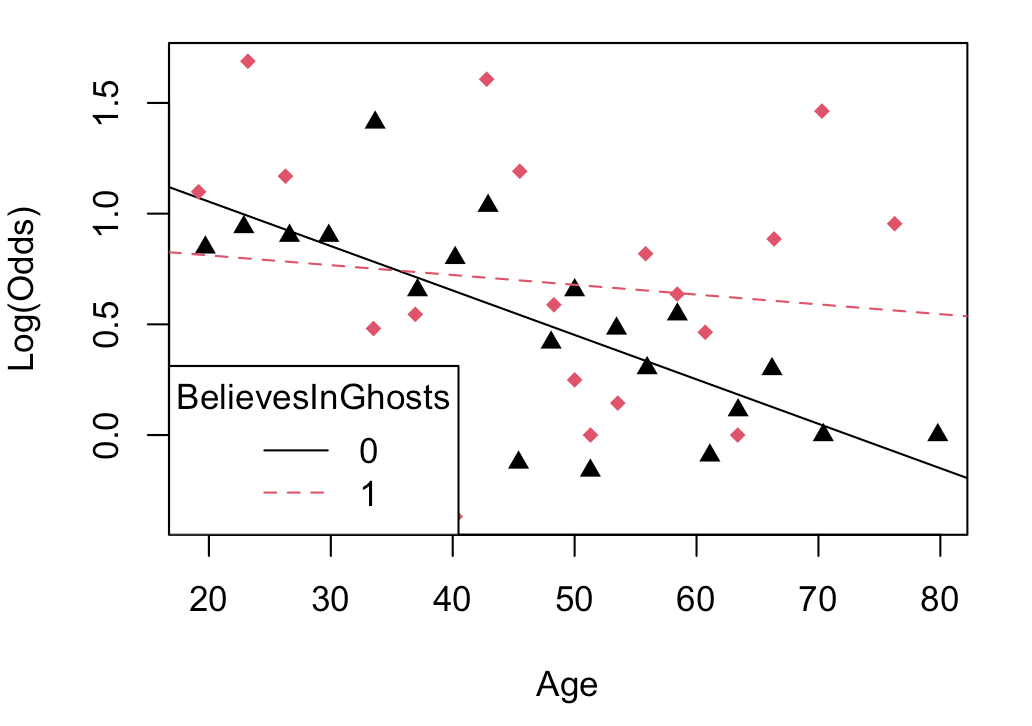
\includegraphics[scale=.3]{intxplot_age_ghosts.png}
    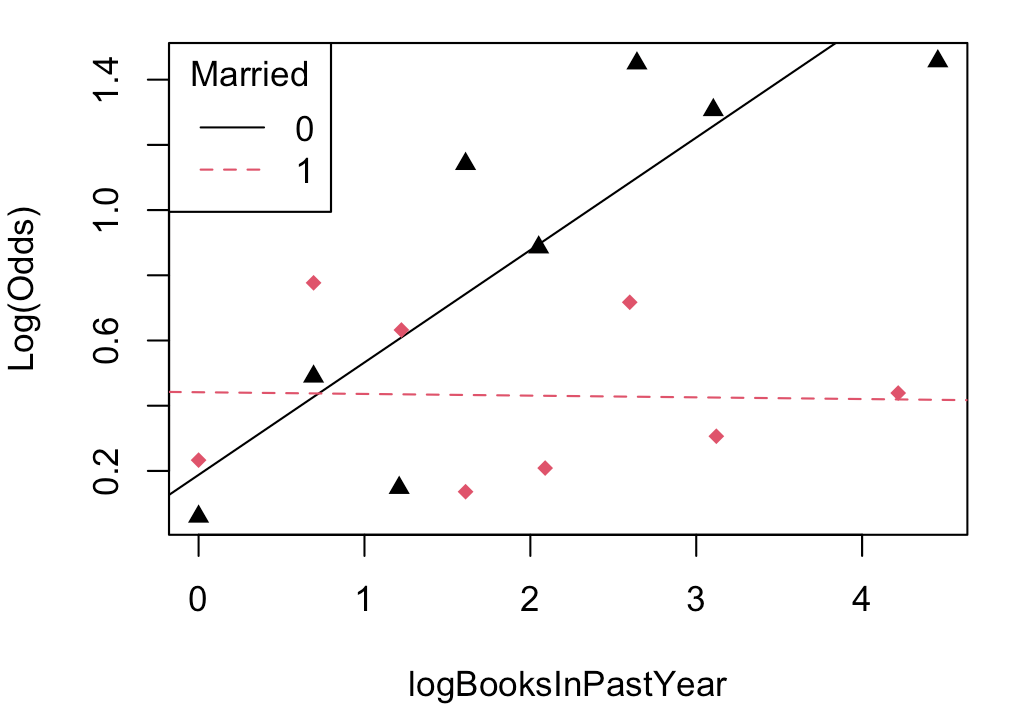
\includegraphics[scale=.3]{intxplot_logbooks_married.png}
    \caption{Significant-looking empirical logit plots of $Age$ and $log(BooksInPastYear)$ split by binary variables}
    \label{fig:EDA_intx}
\end{figure}

\newpage

\subsection{Model Development}

\par To whittle down our variables into a suitable subset, we employ several methods. First, we run a backward step function on the full model, including all our terms and the four possible interactions we identified. This function identifies the least significant variable in the set, then checks if  Akaike's Information Criterion (AIC)\footnote{AIC is a balanced measurement of a model's goodness of fit. It increases with more variables and decreases with smaller residual deviance, so smaller AIC values generally indicate better models.} a  for the model without that variable is significantly higher. If it is, the step function drops that variable. It repeats this process until the increase in AIC is statistically significant.

\par \bigskip Our backward stepwise function on the full set returns a model with many variables: $Age$, $log(BooksInPastYear)$, $Male$, $Married$, $HasSeenTransformers$, $ScientistsGood$, $SmartSadDumbHappy$, $Age:HasSeenTransformers$, and $log(BooksInPastYear):Married$. Running this model confirms that almost every variable is indeed significant at level $\alpha = .05$. The exceptions are $Married$, which is significant at $\alpha = .1$, and the intercept, which is insignificant. The AIC for this model is 783.49, and the residual deviance is 763.49. The null deviance is 855.94, so this model provides a decent reduction in deviance. While the size of this model is remarkable, we may ultimately want to choose a more simple model if its predictive power is similar to this one.

\par \bigskip We also run a forward stepwise function, which starts with the null model including only the intercept, adds the most significant term, checks that AIC was reduced significantly, and repeats until a fully significant set is found. The forward step returns a smaller model that includes $ScientistsGood$, $SmartSadDumbHappy$, $Age$, $Male$, $JobWillBeAutomated$, and $log(BooksInPastYear)$. We run a summary of this model and see that $log(BooksInPastYear)$ is not actually significant; removing it, we obtain a 5-term model with full significance besides the intercept. Its AIC is 793.42 and its residual deviance is 781.42. 

\par \bigskip The R function \texttt{bestglm()} offers a third way of testing our predictors all at once, based on BIC, a different criterion than AIC. At first, \texttt{bestglm()} returns a model with three predictors: $ScientistsGood$, $SmartSadDumbHappy$, and $Age:Male$. We check the summary of this model and see that each variable is highly significant. However, when we use interaction terms, we should include both original variables in the model. Checking the model using these variables plus $Age$ and $Male$, we see that those terms are not significant, and neither is $Age:Male$ with them included. While this interaction is intriguing, we cannot use it.

\par \bigskip Removing $Age:Male$ from the input, we run \texttt{bestglm()} again, which returns a model including $ScientistsGood$, $SmartSadDumbHappy$, $log(BooksInPastYear)$, and $log(BooksInPastYear):Married$. Throwing $Married$ into the mix, we run this model and find that all but $Married$, including the intercept, are significant at level $\alpha = .01$. This model has an AIC of 793.78 and a residual deviance of 781.78. Despite $Married$ being insignificant, this model is promising due to its simplicity and the fact that the intercept is significant.

\subsection{Model Selection}

We now have three models under consideration, each with their own merits.

\begin{center}
    $\text{Model 1: } log(odds) = \beta_0 + \beta_1 ScientistsGood + \beta_2 SmartSadDumbHappy$
    $+ \beta_3 Age + \beta_4 log(BooksInPastYear) + \beta_5 Male + \beta_6 Married + \beta_7 HasSeenTransformers$
    $+ \beta_{37} Age:HasSeenTransformers + \beta_{46} log(BooksInPastYear):Married + \varepsilon$


    \bigskip $\text{Model 2: } log(odds) = \beta_0 + \beta_1 ScientistsGood + \beta_2 SmartSadDumbHappy + \beta_3 Age$
    $+ \beta_4 Male + \beta_5 JobWillBeAutomated + \varepsilon$


    \bigskip $\text{Model 3: } log(odds) = \beta_0 + \beta_1 ScientistsGood + \beta_2 SmartSadDumbHappy + \beta_3 Age$
    $+ \beta_4 log(BooksInPastYear) + \beta_5 Married + \beta_{45} log(BooksInPastYear):Married + \varepsilon$
\end{center}

\par \bigskip To help make our final decision, we will run them as training models on a subset of our data, then see how accurately they can predict whether the remaining subjects believe in anthropogenic climate change. 

\par \bigskip We first randomly sample the integers from 1 to 656, the number of observations in the full dataset, 500 times without repeats. We designate the subset of our data with those row indices our training set. After finding the coefficients for our three models with the training set, we use the models to obtain $log(odds)$ for the 156 remaining observations, then convert the $log(odds)$ to probabilities of belief in anthropogenic climate change.

\par \bigskip Now that we have our predictions, how do we assess their accuracy? Consider the observations for which a model returns a probability greater than 0.5; if the value of $AnthClimateChange$ for that row is 1, we could consider it a ``correct" prediction. We can consider a prediction ``correct" also if our probability guess is less than 0.5 and $AnthClimateChange = 0$. Unfortunately, this measurement does not give us the entire picture about our model accuracy. For instance, it does not measure how strong (i.e. far from 0.5) the predicted probabilities are. That said, it is still a useful measure of our model accuracy.

\par \bigskip If we count up the number of ``correct" predictions for each model and divide them by 156, we get the proportion of ``correct" guesses for each model. After resampling the training set and repeating the process 1000 times, we obtain three 1000-length vectors of these accuracy proportions. Figure \ref{fig:train_histplots} displays histograms of these three vectors. Seeing that their distributions are unimodal and fairly symmetrical, we can safely assume that their means are a good representation of the true accuracy proportions for the three models.

\begin{figure}[h]
    \centering
    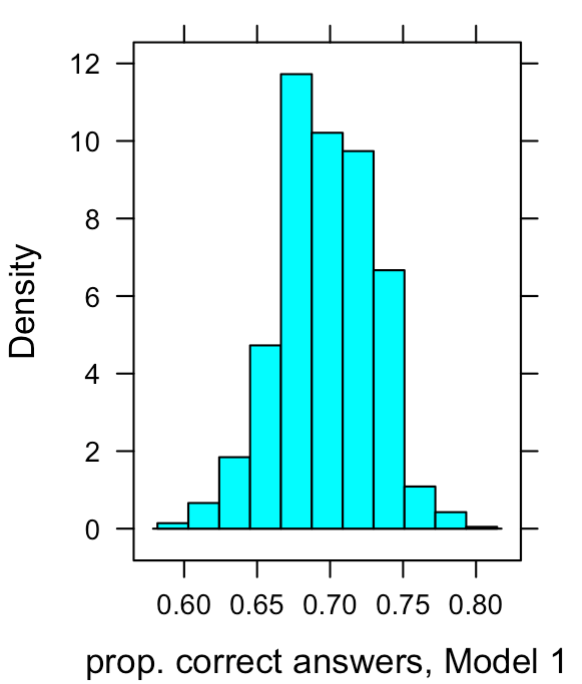
\includegraphics[scale=.45]{histplot_propcorrect1.png}
    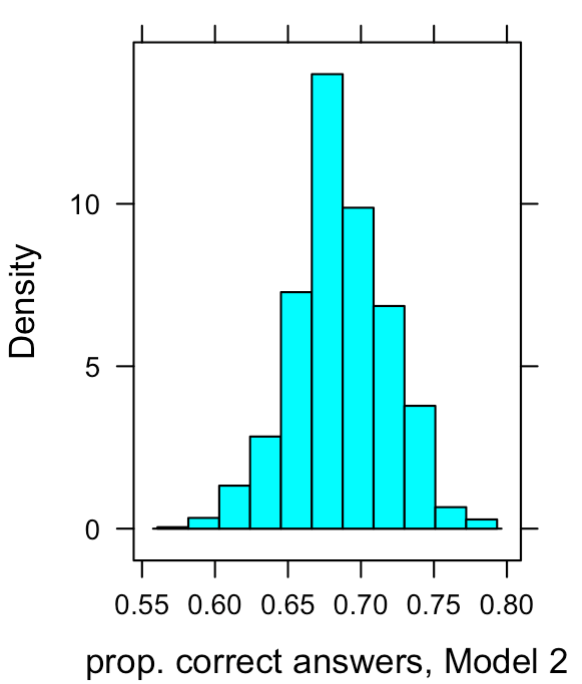
\includegraphics[scale=.45]{histplot_propcorrect2.png}
    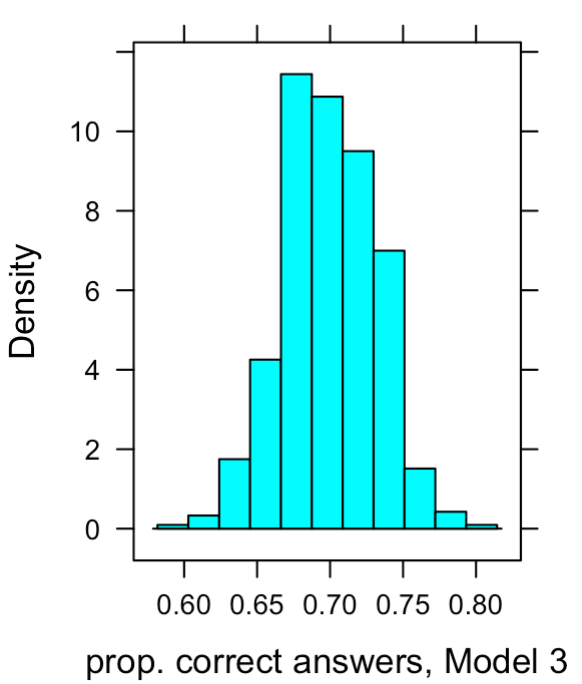
\includegraphics[scale=.45]{histplot_propcorrect3.png}
    \caption{Histogram plots for the proportion of correct guesses made by the three models}
    \label{fig:train_histplots}
\end{figure}

\par \bigskip Running the whole process a few times, we obtain means that average to 0.697 for Model 1, 0.686 for Model 2, and 0.699 for Model 3. These proportions are clearly very similar and our decision is not much easier. We might be inclined to eliminate Model 1 from consideration because it is much more complex than the others, but its AIC, which is designed to punish complexity, is the lowest of the three. Also, complexity might be good for certain purposes because each variable is a new opportunity to differentiate individuals from each other.

\par \bigskip Perhaps controversially, the author decides to publish results for all three models. Each one is simply too interesting to ignore.

\subsection{Checking Conditions}

\par Logistic regression models are valid when their variables (a) are random, (b) are independent, and (c) have a linear relationship with the $log(odds)$ returned. We conclude that condition (a) is satisfied because the survey was conducted by a reputable firm using sound randomization procedures.

\par \bigskip To check condition (b), we find the correlation coefficients between each of the variables in our three models. We see relatively high values for $cor(log(BooksInPastYear)$, $SmartSadDumbHappy)$, $cor(log(BooksInPastYear),Male)$, $cor(Age,HasSeenTransformers)$, and $cor(Age,Married)$, though none are greater than 0.33. Pearson's correlation test tells us that all four correlations are highly significant, calling Models 1 and 3 into question but not Model 2, which does not include any of those variable combinations.

\par \bigskip We can check the collinearity of our models individually with the variance inflation factor (VIF) of each variable other than the interaction terms, which we expect to be correlated with the original terms. Doing so, we find VIFs very close to 1 for all three models and decide that independence is a reasonable-enough assumption for each.

\par \bigskip Finally, we check condition (c). Binary variables necessarily have a linear relationship with $log(odds)$ because there are only two possible values of $log(odds)$. Shown in Figure \ref{fig:conditions_linearity}, plots of $log(odds)$ against our two quantitative variables display fairly linear relationships, though some points stray from the estimated linear function. We conclude that all our conditions are sufficient for each model.

\begin{figure}[h]
    \centering
    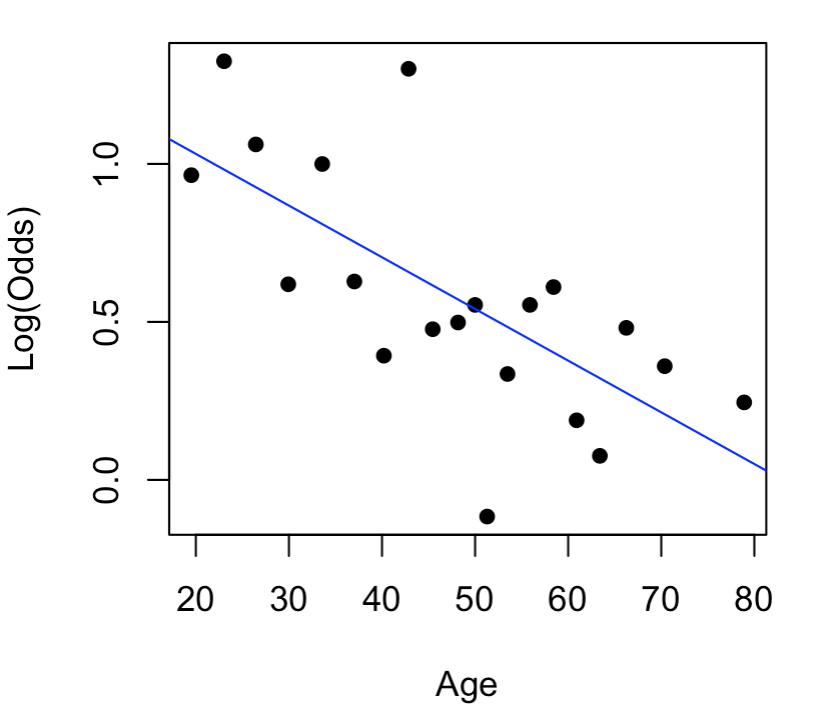
\includegraphics[scale=.5]{linplot_age.png}
    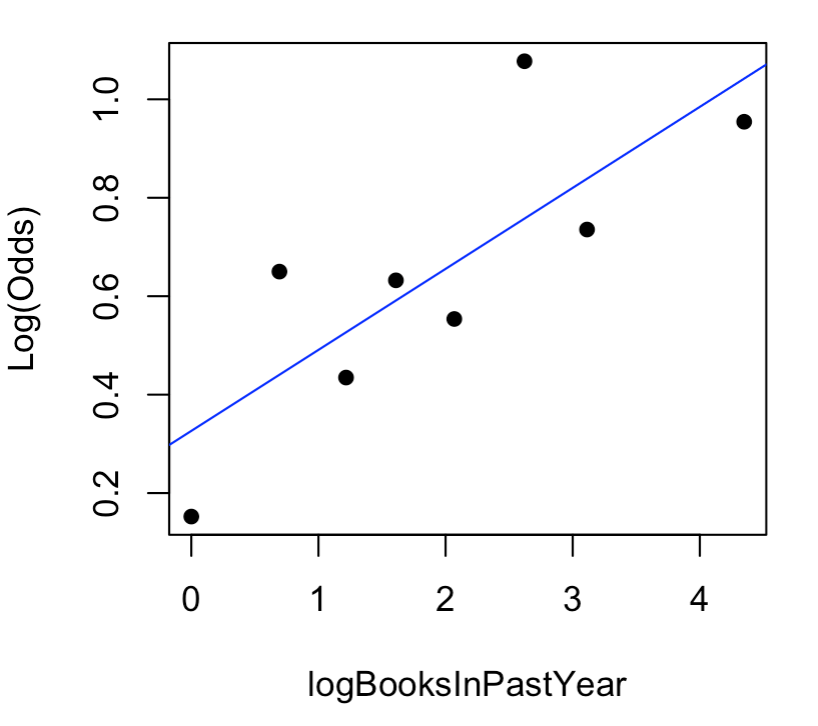
\includegraphics[scale=.5]{linplot_logbooks.png}
    \caption{Plots of $log(odds)$ against $Age$ and $log(BooksInPastYear$}
    \label{fig:conditions_linearity}
\end{figure}